\documentclass[10pt]{article}
\usepackage[english]{babel}

% \usepackage{amsmath, amssymb}
\usepackage{graphicx}
\usepackage{fancyhdr}
\usepackage{url}

\usepackage{caption}
\usepackage{subcaption}

\usepackage{tikz}
\usepackage{amsmath}
\usetikzlibrary{arrows}
\usepackage{verbatim}

\pagestyle{fancy}

\makeatletter

\begin{document}

\begin{titlepage}
\thispagestyle{plain}

\begin{center}
	
\includegraphics[scale=0.12]{unitnlogo}	\\
	University of Trento	\\
	\small {Department of Computer Science}	\\[1cm]
\end{center}

{\centering
\textbf{\Huge An algorithm implementation for Global Predicate Evaluation}\\[1cm]
% \small{Project for the “Distributed Algorithms” course}\\
\small{Trento, 29/08/2016}	\\[1cm]
\textbf{Zen Roberto \& Bof Michele}

}
\vfill

\section*{Abstract}

One core problem in distributed computing is to detect wheter a particular state in a computation can be reached and need to be detected. Problems such as deadlocks detection, monitoring or debugging can be all seen as an instance of the so called Global Predicate Evaluation (GPE) problem. This problem consists in evaluate wheter a given condition called predicate is satisfied among the consistent global states of the system. In order to solve it, one has to face all the practical issues that may arise in a distributed computation: asynchrony and failures of the underlying distributed system, message ordering and inconsistent observations. In this work, we present an implementation that solves GPE based on a simulation of a distributed system. The model built is based on message passing between peers and a monitor which passively observe the system in order to build its global states.


\end{titlepage}


\vspace{3cm}

\section{Introduction}

There is a large class of problems that consist in detecting wheter a particular state in a computation can be reached and need to be detected.
All of those problems can be considered as subclasses of a well known abstract problem in distributed systems called \textit{Global Predicate Evaluation} (GPE). Its goal is to determine whether the global state of a distributed system satisfies some predicate $\Phi$. Those predicates might be related to the state of the system itself such as the possibility of detecting a deadlock or might be related to the state of the computation that is running among a set of processes. A point in common that all those subclasses have is that all those problems or properties can be encoded in terms of variables. GPE consists in evaluate a predicate over them, so compare the value that those variable have with respect to a given condition. There are two different strategies for solving GPE: one is based on a process called monitor, which actively queries the other processes in order to gather enough information to evaluate the predicate; the other strategy is also based on a monitor that passively observes the system and waits for notification of events sent by other processes whenever those events are related to the given predicate. Chose one or the other strategy depends on the underlying distributed system, the communication channels, and more.

In order to inform the monitor about variable changes, processes need to send messages. These messages have to contain at least information related to the predicate that has to be evaluated. However, this is not the only information they need to carry on. Based on the synchrony or the asynchrony of the model one has to keep into consideration problems that may happen such as message ordering beetween a process and the monitor or between processes themselves, messages delays, faulty processes and so on. Hence, there is the need to consider time that can be globally accessed or local to each process. Different time measures for events are considered in solving the GPE: global clock, logical clocks and vector clocks.

We developed a solution to the GPE problem based on a monitor that passively observes the distributed computation and receives messages from peers. Messages are labeled with a vector clock and contain information related to the predicate that the user wants to evaluate. A simulation is started and messages are exchanged randomly between peers which can also execute randomly local events. Once the simulation ends, the monitor collects the histories of events from all the peers, organize them into a \textit{partially ordered set} (poset) and build a lattice in such a way that the user can see it graphically. An analysis of the lattice is done considering that the unstable praticate can be analized in all the possible runs of the lattice (Definitely) or in at least one observation (Possibly).


\newpage

\subsection{Goals}

The reasons which have motivated our group to conduct a study on this topic and the objectives which we have set ourselves are the following:
\begin{enumerate}
\item \textbf{Simulate a distributed computation}. Structure the project in such a way that an user can define how the simulation has to be executed and how long it has to last.
\item \textbf{Develop an application as dinamic as possible}. Allow users to define how many peers will run over the system and their behaviour: establish the probability of executing an internal event rather than a message exchange.
\item \textbf{Evaluate a Global Predicate among all the consistent global states}. Collect only consistent global states so the monitor can evaluate a given predicate over them.
\item \textbf{Display a lattice of the computations}. Display the events executed during the simulation in a lattice so the user can see all the possible runs that could have been executed and the states satisfying the given predicate.
\end{enumerate}

\subsection{Results}

We developed a simple solution to the GPE problem based on a random simulation of distrubuted computations. The project has been develop in Java using JDK version's $1.7$ in combination with the Akka framework which allowed us to build an highly concurrent, distributed, and resilient message-driven application\footnote{\url{http://akka.io}}. We started implementing the behaviour of the peers and then we defined the message exchange between them. In particolar, we adopted a simple strategy for structure messages in a way that they were able to transport all the information needed at the very end of the simulation. To conclude, we defined the behaviour of the monitor such that it is able first to collect all the messages exchanged between the peers and second to evaluate a given predicate over them, taking into consideration only consistend global states stored in a lattice of events.

\subsection{Outline}

The outline of this report is structured as follows. Section 2 describes the problem of GPE, as one of the core problem in distributed system. Section 3 explains details about the solution we propose, the problems we faced, the strategies and assumptions we adopted to overcome them. In this section we do not go deep into the implementation details, instead we will focus on the logics behind our strategies. In Section 4 we will show some experimental evaluations of our implementation. The last section states the conclusion of our work and ideas on how we could improve our solution with techniques based on high-level operators that run in parallel.

\section{The Solution}

We developed an application using the Akka framework which emphasises the concept of \textit{actors} as entities that may make local decisions, execute events or send messages to other actors. Our solution is based on the fact that a user can specify the duration of the distributed computation and the behaviour of the actors in the system. In our implementatio, actors are are both peers and monitor who take place in the simulation and interact each other use purely message passing. An important note is that everything in Akka is asynchronous\footnote{\url{http://doc.akka.io/docs/akka/2.4/general/remoting.html}}.

Altough it is a very simple implementation for solving the GPE problem, different options on how to develop our project were considered. We started developing a real P2P system by running peers for a period of time equal to the one specified by the user. Once this period of time elapsed, the peers send all their history of events to the monitor which evaluates a given predicate on the global states built.

The problem we faced developing this solution was that if the user specifies a period of time long enough, no evaluation is performed until this time elapses. Hence, the user has the costraint of waiting for a period of time equal to the one he specified.

Based on the problem stated above, we decided to refine our implementation and we developed a simulated distributed system. As before, the user specifies the duration of the simulation. However, rather than running peers for a well known period of time, each peer simulates its behaviour during a period of time equal to the one specified by scheduling events in the future. As soon as the last scheduled event is far away in the future from the end of the simulation, the peers simulation ends and the history of events collected is sent to the monitor. In addition, as soon as the monitor collects messages and evaluates a predicate over the consistent global states collected, the execution ends. In this way, we allow users to simulate a long distributed computation without waste his time.

\subsection{Assumptions}

We decided to work under an asynchronous system, the weakest possible model for a distributed network, because it enables us to estabilish upper bounds on the cost of solving problems in distributed systems\cite{Babaoglu}. Because we are dealing with this model we have to deal with the problems that might arise during the execution of distributed computations. In fact, those systems rule out the possibility of processes to maintaining syncronized local clocks so communication remains the only possible mechanism for synchronization in such systems. However, there are no bounds on the relative speeds of processes and there exist no bounds on message delays. Hence, in order to assure that the project works on those systems, we posed the following assumptions for the underlying system and the communication:

\begin{enumerate}
\item \textbf{Actors are correct}. Both the peers and the monitor are correct: actors cannot be faulty so they cannot fail or behaviour in a bizantine way.
\item \textbf{The communication network is strongly connected}. Every peer can communicate directly with every other peer.
\item \textbf{Messages sent are at-most-once delivered}. Based on the Akka framework, at-most-once delivery means that for each message handed to the mechanism, that message is delivered zero or one times; it means that messages may be lost.
\item \textbf{Message ordering is mantained per sender-receiver pair}. For a given pair of actors, messages sent directly from the first to the second will not be received out-of-order. Hence, message buffers between pair of actors are FIFO.
\end{enumerate}

\subsection{Initialization}

Each simulation starts by executing the \textit{Simulator} class. Firstly, it acquires the configuration specified by the user such as the number of peers in the actual system, the duration of the simulation and more. Secondly, it creates an actor system which generates the peers and the monitor as its children, and then sends a \textit{StartMessage} to them in order to initialize the actors. When the monitor receives the \textit{StartMessage} it starts listening and waiting for \textit{EndMessages} sent by all the peers at the end of their simulation. On the other hand, once a peer received a \textit{StartMessage} it initializes its vector clock and it can start sending messages to its neighbours.
Although this is a simple protocol in which StartMessages and EndMessages estabilish respectively the start and the end of the simulation, it is not difficult to understand that this procedure may cause problems. In order to explain what may happen, let's describe it in a scenario.

\vspace{0.2cm}
\emph{``Suppose that the actors in the system are two peers and the monitor. The actor system sends a StartMessage to all of them but due to the asynchrony of the underlying distributed system, one of the message sent to a peer is delayed. The peer who received the message first initialize its vector clock and start sending messages to the other peer who does not received yet the StartMessage. If the receipient peer received the message from the peer before the StartMessage sent by the monitor arrived, it cannot update its vector clock because it was not initialized before.''}
\vspace{0.1cm}

\tikzstyle{every picture}+=[remember picture]
\everymath{\displaystyle}
\begin{figure}[ht!]
\centering
\scalebox{.8}{
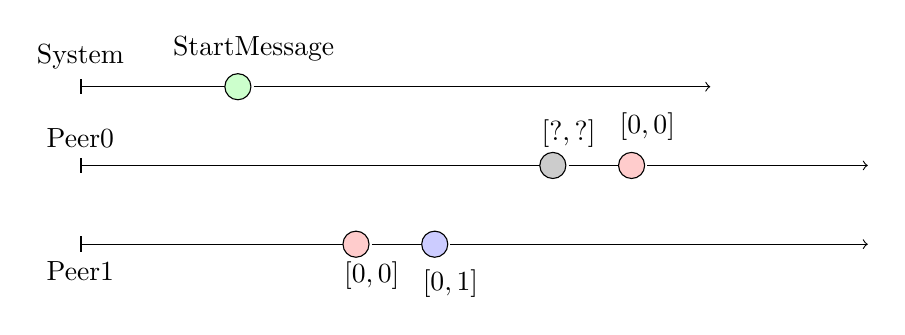
\begin{tikzpicture}

% SYSTEM
\draw[|-] (0,2) node[above=1mm]{System} -- (2,2) node{\tikz[baseline]{
	\node[fill=green!20,draw,circle] (sm){};
}};
\draw[->] (2.2,2) node[above=2mm]{StartMessage} -- (8,2) {};

% PEER 0
\draw[|-] (0,1) node[above=1mm]{Peer0} -- (6,1) node{\tikz[baseline]{
	\node[fill=black!20,draw,circle] (f0){};
}};
\draw[-] (6.2,1) node[above=1mm]{$[?,?]$} -- (7,1) node{\tikz[baseline]{
	\node[fill=red!20,draw,circle] (f1){};
}};
\draw[->] (7.2,1) node[above=2mm]{$[0,0]$} -- (10,1) node[below=1mm]{};

% PEER 1
\draw[|-] (0,0) node[below=1mm]{Peer1} -- (3.5,0) node{\tikz[baseline]{
	\node[fill=red!20,draw,circle] (e0){};
}};
\draw[-] (3.7,0) node[below=1mm]{$[0,0]$} -- (4.5,0) node{\tikz[baseline]{
	\node[fill=blue!20,draw,circle] (e1){};
}};
\draw[->] (4.7,0) node[below=2mm]{$[0,1]$} -- (10,0) node[below=1mm]{};

\end{tikzpicture}

\begin{tikzpicture}[overlay]
  \path[->] (sm) edge [out=-90, in=135] (e0);
  \path[->] (sm) edge [out=-45, in=135] (f1);
  \path[->] (e1) edge [out=45, in=-135] (f0);
\end{tikzpicture}
}

\caption{An overcomed issue in our asyncronous simulation.}
\label{fig:worst_case}
\end{figure}


\noindent
Figure \ref{fig:worst_case} shows the problem described in the above scenario. StartMessages are sent by the system actor but one of them arrives earlier than the other. Between the two events a message is exchanged and the update of a vector clock is not possible. We overcomed this problem with a simple solution based on the notion of \textit{common knowledge}: ``we want the other know that I am ready to start send messages''.

\pagestyle{empty}
\tikzstyle{every picture}+=[remember picture]
\everymath{\displaystyle}
\begin{figure}[!ht]
\centering
\scalebox{.8}{

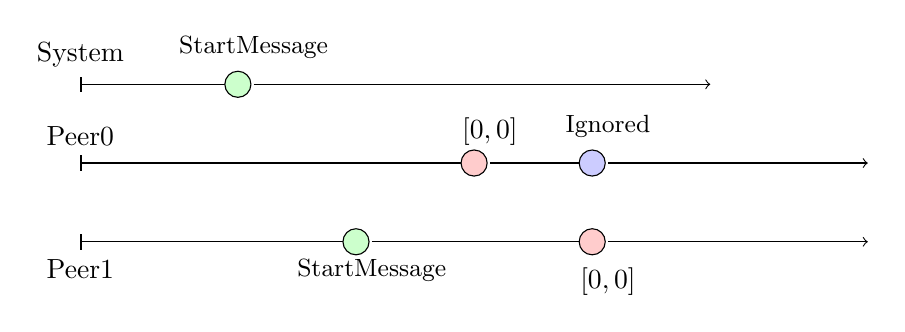
\begin{tikzpicture}

% SYSTEM TIMELINE
\draw[|-] (0,2) node[above=1mm]{System} -- (2,2) node{\tikz[baseline]{
	\node[fill=green!20,draw,circle] (sm){};
}};
\draw[->] (2.2,2) node[above=2mm]{\small{StartMessage}} -- (8,2) {};

% PEER 0
\draw[|-] (0,1) node[above=1mm]{Peer0} -- (5,1) node{\tikz[baseline]{
	\node[fill=red!20,draw,circle] (f0){};
}};
\draw[-] (5.2,1) node[above=1mm]{$[0,0]$} -- (6.5,1) node{\tikz[baseline]{
	\node[fill=blue!20,draw,circle] (f1){};
}};
\draw[->] (6.7,1) node[above=2mm]{\small{Ignored}} -- (10,1) node[below=1mm]{};

% PEER 1
\draw[|-] (0,0) node[below=1mm]{Peer1} -- (3.5,0) node{\tikz[baseline]{
	\node[fill=green!20,draw,circle] (e0){};
}};
\draw[-] (3.7,0) node[below=1mm]{\small{StartMessage}} -- (6.5,0) node{\tikz[baseline]{
	\node[fill=red!20,draw,circle] (e1){};
}};
\draw[->] (6.7,0) node[below=2mm]{$[0,0]$} -- (10,0) node[below=1mm]{};

\end{tikzpicture}

\begin{tikzpicture}[overlay]
    \path[->] (sm) edge [out=-90, in=135] (e0);
    \path[->] (sm) edge [out=-45, in=135] (f1);
    \path[->] (e0) edge [out=45, in=-135] (f0);
    \path[->] (f0) edge [out=-45, in=135] (e1);
\end{tikzpicture}

}

  \caption{An issue overcomed in our asyncronous simulation.}
\end{figure}


\noindent
Figure \ref{fig:worst_case_solved} displays how we solved the problem related to Figure \ref{fig:worst_case}. The first time a StartMessage is received, each peer initializes its vector clock and sends a StartMessage to everybody else in order to share common knowledge. This procedure is executed only once, the other StartMessages received are ignored. The assumptions made in Section 2 allow us to reason about the correctness of this protocol because message ordering is mantained per sender-receiver pair.


\subsection{The simulation}

\begin{figure}[ht]
	\centering
	\begin{minipage}{.5\textwidth}
	  \scalebox{.8}{\pagestyle{empty}
\tikzstyle{every picture}+=[remember picture]
\everymath{\displaystyle}

\begin{figure}[!ht]

\centering
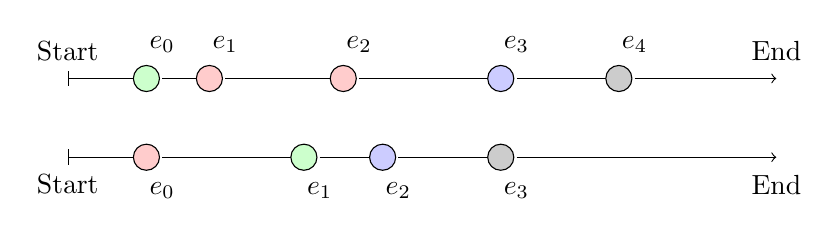
\begin{tikzpicture}

% FIRST TIMELINE

\draw[|-] (1,0) node[below=1mm]{Start} -- (2,0) node{\tikz[baseline]{
	\node[fill=red!20,draw,circle] (e0){};
}
};
\draw[-] (2.2,0) node[below=2mm]{$e_0$} -- (4,0) node{\tikz[baseline]{
	\node[fill=green!20,draw,circle] (e1){};
}
};
\draw[-] (4.2,0) node[below=2mm]{$e_1$} -- (5,0) node{\tikz[baseline]{
	\node[fill=blue!20,draw,circle] (e2){};
}
};
\draw[-] (5.2,0) node[below=2mm]{$e_2$} -- (6.5,0) node{\tikz[baseline]{
	\node[fill=black!20,draw,circle] (e3){};
}
};
\draw[->] (6.7,0) node[below=2mm]{$e_3$} -- (10,0) node[below=1mm]{End};

% SECOND TIMELINE

\draw[|-] (1,1) node[above=1mm]{Start} -- (2,1) node{\tikz[baseline]{
	\node[fill=green!20,draw,circle] (f0){};
}
};
\draw[-] (2.2,1) node[above=2mm]{$e_0$} -- (2.8,1) node{\tikz[baseline]{
	\node[fill=red!20,draw,circle] (f1){};
}
};
\draw[-] (3,1) node[above=2mm]{$e_1$} -- (4.5,1) node{\tikz[baseline]{
	\node[fill=red!20,draw,circle] (f2){};
}
};
\draw[-] (4.7,1) node[above=2mm]{$e_2$} -- (6.5,1) node{\tikz[baseline]{
	\node[fill=blue!20,draw,circle] (f3){};
}
};
\draw[-] (6.7,1) node[above=2mm]{$e_3$} -- (8,1) node{\tikz[baseline]{
	\node[fill=black!20,draw,circle] (f4){};
}
};
\draw[->] (8.2,1) node[above=2mm]{$e_4$} -- (10,1) node[above=1mm]{End};

\end{tikzpicture}

% Now it's time to draw some edges between the global nodes. Note that we
% have to apply the 'overlay' style.
\begin{tikzpicture}[overlay]
        \path[->] (f0) edge [out=-90, in=135] (e1);
        \path[->] (e2) edge [out=45, in=-135] (f3);
        \path[->] (e3) edge [out=45, in=-135] (f4);
\end{tikzpicture}

  \caption{An example of a simulation. Red circles are peers' internal events.}
\end{figure}
}
	\end{minipage}%
	\begin{minipage}{.5\textwidth}
	  \scalebox{.8}{\pagestyle{empty}
\tikzstyle{every picture}+=[remember picture]
% \everymath{\displaystyle}
% \begin{figure}[!ht]

\centering
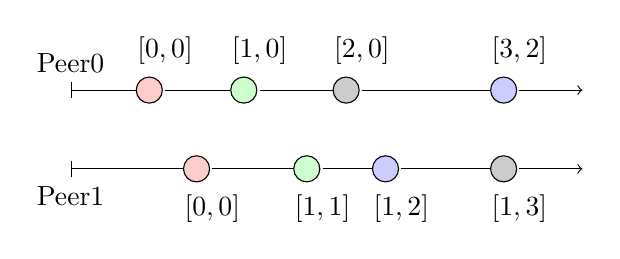
\begin{tikzpicture}

% PEER 0
\draw[|-] (0,1) node[above=1mm]{Peer0} -- (1,1) node{\tikz[baseline]{
	\node[fill=red!20,draw,circle] (f0){};
}};
\draw[-] (1.2,1) node[above=2mm]{$[0,0]$} -- (2.2,1) node{\tikz[baseline]{
	\node[fill=green!20,draw,circle] (f1){};
}};
\draw[-] (2.4,1) node[above=2mm]{$[1,0]$} -- (3.5,1) node{\tikz[baseline]{
	\node[fill=black!20,draw,circle] (f2){};
}};
\draw[-] (3.7,1) node[above=2mm]{$[2,0]$} -- (5.5,1) node{\tikz[baseline]{
	\node[fill=blue!20,draw,circle] (f3){};
}};
\draw[->] (5.7,1) node[above=2mm]{$[3,2]$} -- (6.5,1) node{};

% PEER 1
\draw[|-] (0,0) node[below=1mm]{Peer1} -- (1.6,0) node{\tikz[baseline]{
	\node[fill=red!20,draw,circle] (e0){};
}};
\draw[-] (1.8,0) node[below=2mm]{$[0,0]$} -- (3,0) node{\tikz[baseline]{
	\node[fill=green!20,draw,circle] (e1){};
}};
\draw[-] (3.2,0) node[below=2mm]{$[1,1]$} -- (4,0) node{\tikz[baseline]{
	\node[fill=blue!20,draw,circle] (e2){};
}};
\draw[-] (4.2,0) node[below=2mm]{$[1,2]$} -- (5.5,0) node{\tikz[baseline]{
	\node[fill=black!20,draw,circle] (e3){};
}};
\draw[->] (5.7,0) node[below=2mm]{$[1,3]$} -- (6.5,0) node[below=1mm]{};
\end{tikzpicture}

\begin{tikzpicture}[overlay]
	\path[->] (f1) edge [out=-90, in=135] (e1);
	\path[->] (e2) edge [out=45, in=-135] (f3);
\end{tikzpicture}

  % \caption{An example of a simulation. Red circles are peers' internal events.}
% \end{figure}
}
	\end{minipage}
\end{figure}

\tikzstyle{every picture}+=[remember picture]
\everymath{\displaystyle}
\begin{figure}[!ht]

\hspace{0.5cm} Events:
\([ \thinspace
\tikz\node [fill=red!20,draw,circle] (n1) {}; \thinspace
\tikz\node [fill=green!20,draw,circle] (n2){}; \thinspace
\tikz\node [fill=blue!20,draw,circle] (n3) {}; \thinspace
\tikz\node [fill=black!20,draw,circle] (n4){}; \thinspace
]
\vspace{1cm}
\)

\centering
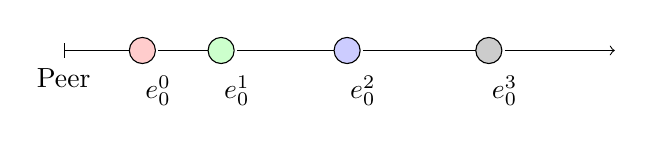
\begin{tikzpicture}
\draw[|-] (1,0) node[below=1mm]{Peer} -- (2,0) node{\tikz[baseline]{
	\node[fill=red!20,draw,circle] (e0){};
}};
\draw[-] (2.2,0) node[below=2mm]{$e^0_0$} -- (3,0) node{\tikz[baseline]{
	\node[fill=green!20,draw,circle] (e1){};
}};
\draw[-] (3.2,0) node[below=2mm]{$e^1_0$} -- (4.6,0) node{\tikz[baseline]{
	\node[fill=blue!20,draw,circle] (e2){};
}};
\draw[-] (4.8,0) node[below=2mm]{$e^2_0$} -- (6.4,0) node{\tikz[baseline]{
	\node[fill=black!20,draw,circle] (e3){};
}};
\draw[->] (6.6,0) node[below=2mm]{$e^3_0$} -- (8,0) node[below=1mm]{};
\end{tikzpicture}

\begin{tikzpicture}[overlay]
        \path[->] (n1) edge [out=-90, in=120] (e0);
        \path[->] (n2) edge [out=-90, in=120] (e1);
        \path[->] (n3) edge [out=-70, in=135] (e2);
        \path[->] (n4) edge [out=-60, in=135] (e3);
\end{tikzpicture}

  \caption{The sequence of events stored in the peer list's and scheduled in the time space diagram.}
	\label{fig:events}
\end{figure}


Non laborum excepteur sint sunt aute esse aliquip. Velit irure ea culpa nulla id mollit laboris laboris adipisicing ipsum non do in id aute anim cupidatat. Veniam deserunt excepteur commodo eu duis nulla adipisicing anim amet adipisicing ex. Laborum Lorem do nulla sint qui voluptate sint esse in incididunt Lorem cillum voluptate tempor nisi. Mollit voluptate mollit eiusmod anim elit nostrud voluptate veniam commodo id do officia cillum voluptate fugiat cillum. In incididunt proident qui id velit eiusmod aliquip aliqua nulla officia ut. Dolore aute est aliqua qui do eu sunt in est ad aliquip nulla anim deserunt. Ut sunt voluptate consectetur magna ex minim ut magna cillum aliquip elit voluptate ex excepteur eiusmod occaecat.

Non laborum excepteur sint sunt aute esse aliquip. Velit irure ea culpa nulla id mollit laboris laboris adipisicing ipsum non do in id aute anim cupidatat. Veniam deserunt excepteur commodo eu duis nulla adipisicing anim amet adipisicing ex. Laborum Lorem do nulla sint qui voluptate sint esse in incididunt Lorem cillum voluptate tempor nisi. Mollit voluptate mollit eiusmod anim elit nostrud volup.

% \tikzstyle{every picture}+=[remember picture]
\everymath{\displaystyle}
\begin{figure}[ht!]
\centering
\scalebox{.8}{
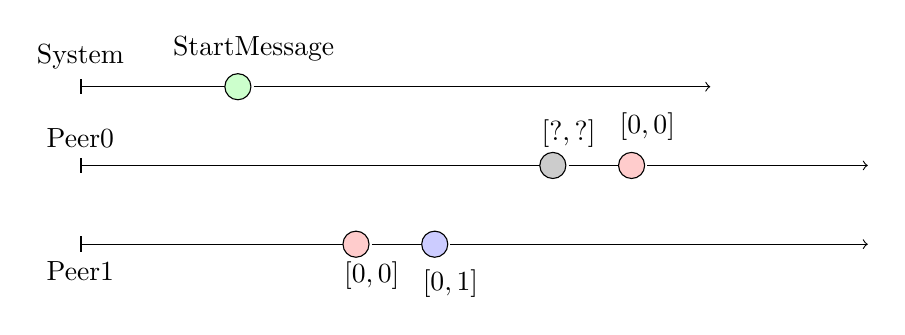
\begin{tikzpicture}

% SYSTEM
\draw[|-] (0,2) node[above=1mm]{System} -- (2,2) node{\tikz[baseline]{
	\node[fill=green!20,draw,circle] (sm){};
}};
\draw[->] (2.2,2) node[above=2mm]{StartMessage} -- (8,2) {};

% PEER 0
\draw[|-] (0,1) node[above=1mm]{Peer0} -- (6,1) node{\tikz[baseline]{
	\node[fill=black!20,draw,circle] (f0){};
}};
\draw[-] (6.2,1) node[above=1mm]{$[?,?]$} -- (7,1) node{\tikz[baseline]{
	\node[fill=red!20,draw,circle] (f1){};
}};
\draw[->] (7.2,1) node[above=2mm]{$[0,0]$} -- (10,1) node[below=1mm]{};

% PEER 1
\draw[|-] (0,0) node[below=1mm]{Peer1} -- (3.5,0) node{\tikz[baseline]{
	\node[fill=red!20,draw,circle] (e0){};
}};
\draw[-] (3.7,0) node[below=1mm]{$[0,0]$} -- (4.5,0) node{\tikz[baseline]{
	\node[fill=blue!20,draw,circle] (e1){};
}};
\draw[->] (4.7,0) node[below=2mm]{$[0,1]$} -- (10,0) node[below=1mm]{};

\end{tikzpicture}

\begin{tikzpicture}[overlay]
  \path[->] (sm) edge [out=-90, in=135] (e0);
  \path[->] (sm) edge [out=-45, in=135] (f1);
  \path[->] (e1) edge [out=45, in=-135] (f0);
\end{tikzpicture}
}

\caption{An overcomed issue in our asyncronous simulation.}
\label{fig:worst_case}
\end{figure}


Mollit consequat ut ut sit labore quis fugiat sunt Lorem velit sint nisi.

% \pagestyle{empty}
\tikzstyle{every picture}+=[remember picture]
\everymath{\displaystyle}
\begin{figure}[!ht]
\centering
\scalebox{.8}{

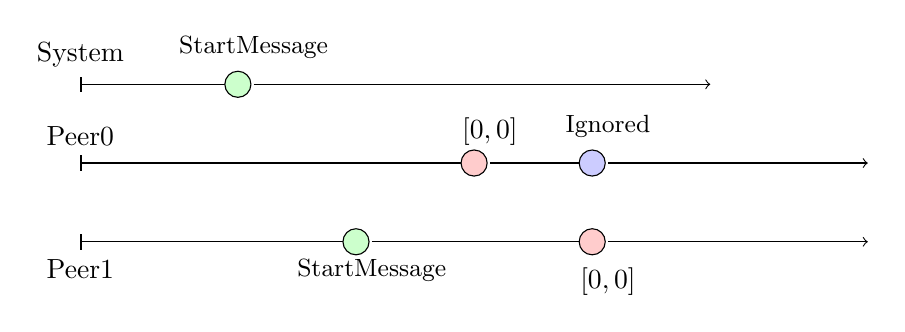
\begin{tikzpicture}

% SYSTEM TIMELINE
\draw[|-] (0,2) node[above=1mm]{System} -- (2,2) node{\tikz[baseline]{
	\node[fill=green!20,draw,circle] (sm){};
}};
\draw[->] (2.2,2) node[above=2mm]{\small{StartMessage}} -- (8,2) {};

% PEER 0
\draw[|-] (0,1) node[above=1mm]{Peer0} -- (5,1) node{\tikz[baseline]{
	\node[fill=red!20,draw,circle] (f0){};
}};
\draw[-] (5.2,1) node[above=1mm]{$[0,0]$} -- (6.5,1) node{\tikz[baseline]{
	\node[fill=blue!20,draw,circle] (f1){};
}};
\draw[->] (6.7,1) node[above=2mm]{\small{Ignored}} -- (10,1) node[below=1mm]{};

% PEER 1
\draw[|-] (0,0) node[below=1mm]{Peer1} -- (3.5,0) node{\tikz[baseline]{
	\node[fill=green!20,draw,circle] (e0){};
}};
\draw[-] (3.7,0) node[below=1mm]{\small{StartMessage}} -- (6.5,0) node{\tikz[baseline]{
	\node[fill=red!20,draw,circle] (e1){};
}};
\draw[->] (6.7,0) node[below=2mm]{$[0,0]$} -- (10,0) node[below=1mm]{};

\end{tikzpicture}

\begin{tikzpicture}[overlay]
    \path[->] (sm) edge [out=-90, in=135] (e0);
    \path[->] (sm) edge [out=-45, in=135] (f1);
    \path[->] (e0) edge [out=45, in=-135] (f0);
    \path[->] (f0) edge [out=-45, in=135] (e1);
\end{tikzpicture}

}

  \caption{An issue overcomed in our asyncronous simulation.}
\end{figure}


Non laborum excepteur sint sunt aute esse aliquip. Velit irure ea culpa nulla id mollit laboris laboris adipisicing ipsum non do in id aute anim cupidatat. Veniam deserunt excepteur commodo eu duis nulla adipisicing anim amet adipisicing ex. Laborum Lorem do nulla sint qui voluptate sint esse in incididunt Lorem cillum voluptate tempor nisi. Mollit voluptate mollit eiusmod anim elit nostrud volup

\section{Evaluation}

\section{Conclusion}

\bibliographystyle{abbrv}
\bibliography{bibliography}

\end{document}
